\label{sec:problema}

\subsection{DUNE, FD3 and scintillation light}
\label{sec:detector}

DUNE (Deep Underground Neutrino Experiment) will study neutrino oscillation with a beam from Fermilab and a far detector \qty{1300}{\km} away; its goals include CP violation (charge conjugation and parity), the mass ordering, supernova neutrinos and proton decay \citep{abi2020volume}. According to \citet{abud2024dunephase}, the far detector uses liquid argon time projection chambers (LArTPCs); Phase~II adds the third module (FD3), a vertical drift module like the second (FD2); the photon detection system of FD3 will be defined by the APEX programme (Aluminum Profiles with Embedded X-ARAPUCA).

Charged particles ionise and excite the argon: the electrons drift to the readout planes, which give the coordinates perpendicular to the drift, and the scintillation (about \num{24000} photons per MeV at \qty{500}{\V\per\cm}, near \qty{127}{\nm}) marks the time $t_0$ of the interaction, on which the drift coordinate depends \citep{abi2020volume}. Supernova neutrinos have energies of the order of \qty{10}{\MeV} \citep{abi2021supernova}; in this regime, the position obtained from the light helps to select the fiducial volume and to reject radiological backgrounds \citep{paulucci2022dune}. Below \qty{5}{\MeV}, the role of light in isolated deposits is little explored \citep{caratelli2022low}.

APEX envisages about \num{7000} X-ARAPUCA photon detectors of \qtyproduct{50 x 50}{\cm} in the field cage profiles, with an optical coverage close to \qty{60}{\percent} \citep{marinho2025apex}; each one shifts the wavelength of the light and traps it until it is detected by silicon photomultipliers \citep{machado2018xarapuca}. Simulated with a detection efficiency of \qty{2}{\percent}, APEX has, in the central region, an average light yield (LY) of \num{180} photoelectrons (p.e.)\ per MeV and a minimum of \qty{109}{\pe\per\MeV}, and a higher LY towards the ends; analytic estimators reconstruct position and energy \citep{marinho2025apex}.

\subsection{Simulated data and photon-counting regime}
\label{sec:dados}

The simulation is that of the previous stage \citep{vicentin2024study}: \num{9364} events with deposited energy $E = {}$\qty{100}{\MeV}. The vertex $\mathbf{v} = (x, y, z)$ is expressed in the sensor frame, used throughout the report; in the file-name frame (Section~\ref{sec:dados_grafos}), it is $\mathbf{t} = (t_x, t_y, t_z)$, and \mbox{$(x, y, z) = (t_y, -t_x, t_z)$}. The vertices form a grid of \numproduct{13 x 12 x 60}~$=$~\num{9360} positions spaced \qty{0.5}{\m} apart (\qty{0.45}{\m} in the first step in $x$), in one octant: $x$ from \num{0.05} to \qty{6.0}{\m}, $y$ from \num{-5.5} to \qty{0}{\m} and $z$ from \num{0} to \qty{29.5}{\m}. Four of these positions have two events. There are \num{6912} channels, at positions $\mathbf{p}_i$: \num{2880} on each long wall ($y = {}$\qty{\pm 6.673}{\m}), \num{576} on each end cap ($z = {}$\qty{\pm 29.93}{\m}) and none on the faces normal to $x$; this total is that of a fully instrumented APEX field cage, \num{192} modules of \num{36} photon detectors \citep{abud2024dunephase}. The long axis, $z$, follows the beam.

A \qty{10}{\MeV} deposit is represented by
\begin{equation}
  \tilde{N}_i = \operatorname{round}(s N_i), \qquad n_i \sim \operatorname{Binomial}(\tilde{N}_i, \varepsilon),
  \label{eq:luz}
\end{equation}
where $N_i$ is the number of photons reaching channel $i$ in the \qty{100}{\MeV} simulation, already corrected (Section~\ref{sec:dados_grafos}); $s = {}$\num{0.1} is the scale factor; $\tilde{N}_i$ is the scaled and rounded count; $\varepsilon = {}$\num{0.02} is the detection efficiency assumed by APEX \citep{marinho2025apex}; and $n_i$ is the number of detected photoelectrons. Each event has one photon draw (seed \num{42} plus its index), shared by all epochs and models.

On average, the test events have \qty{530.1}{\pe} (\qty{53.0}{\pe\per\MeV}) in \num{245} channels. Over the \num{9364} events, on average only \qty{3.6}{\percent} of the channels record light (Figure~\ref{fig:evento_exemplo}); the light per event ranges from \num{43} to \qty{2334}{\pe} and falls with the distance from the vertex to the nearest long wall (Figure~\ref{fig:luz_distancia}); in total, that wall receives \qty{70.2}{\percent} of the photoelectrons, the nearest end cap \qty{20.7}{\percent} and the opposite wall \qty{9.2}{\percent}. With the average yield of APEX, a \qty{10}{\MeV} deposit would give \qty{1800}{\pe}, \num{3.4} times the mean test light, which corresponds to \qty{2.9}{\MeV}, the energy of the comparison at equal detected light (Section~\ref{sec:protocolo_comparacao}).

\begin{figure}[H]
  \centering
  \begin{subfigure}[t]{0.485\textwidth}
    \centering
    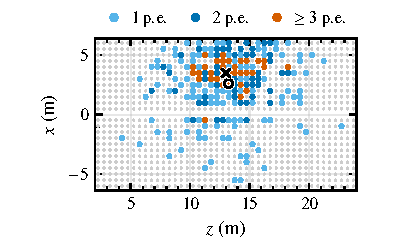
\includegraphics{figures/evento_exemplo.pdf}
    \caption{Long wall at $y = {}$\qty{-6.673}{\m}, the nearest to the vertex, in test event \num{5834} (\qty{387}{\pe} in \num{247} of the \num{6912} channels); it receives most of the light, and all its lit channels are in the part shown. Grey dots: unlit channels; colour: photoelectrons per channel; cross: projection of the vertex; circle: projection of the light centroid, where the global node of the graph sits (Section~\ref{sec:dados_grafos}).}
    \label{fig:evento_exemplo}
  \end{subfigure}\hfill
  \begin{subfigure}[t]{0.485\textwidth}
    \centering
    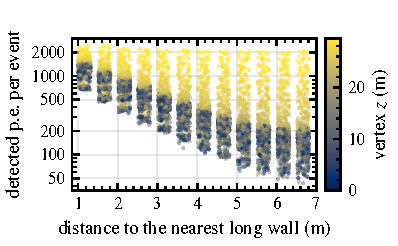
\includegraphics{figures/luz_distancia.pdf}
    \caption{Detected light per event, on a logarithmic scale, for the \num{9364} simulated events, as a function of the distance from the vertex to the nearest long wall; the colour indicates the $z$ coordinate of the vertex. The light falls with distance and is higher near the end cap. The vertices lie at \num{12} distances, \qty{0.5}{\m} apart; the points were shifted at random horizontally to reduce overlap.}
    \label{fig:luz_distancia}
  \end{subfigure}
  \caption{Photon-counting regime: (a) a test event; (b) the light of all simulated events.}
  \label{fig:regime_fotons}
\end{figure}

\subsection{Objective and task formulation}
\label{sec:tarefa}

In the previous stage \citep{vicentin2024study}, a dense network of \num{8195} parameters, fed by \num{60} descriptors selected in phases, obtained a test mean absolute error (MAE) of \num{12.03} to \qty{18.18}{\cm} per axis; since the descriptors summarise the readout of the whole detector, the model receives only what they retain of the light pattern on the channels. This stage represents each event as a graph of the lit channels, estimates the vertex by message passing and compares, on the same test events, \num{11} encoders with almost equal parameter totals (matched capacity), tuned boosters (decision-tree ensembles: XGBoost and LightGBM) and the light barycentre, with the quoted values of the previous network and with APEX at equal detected light. The report also investigates where the error concentrates and what limits it.

The task is to estimate $\mathbf{v}$ from the positions $\mathbf{p}_i$ and the light $n_i$ of the active channels (non-zero $n_i$), which form the set $A$, with $|A|$ elements.

For the predicted vertex $\hat{\mathbf{v}}$ and $J$ events (\num{937} in the test set), the evaluation computes
\begin{equation}
  \begin{aligned}
    \mathrm{MAE}_a &= \bigl\langle \lvert \hat{v}_a - v_a \rvert \bigr\rangle, &\qquad
    \mathrm{RMSE}_a &= \sqrt{\bigl\langle (\hat{v}_a - v_a)^2 \bigr\rangle}, \\
    \mathrm{RMSE}_{\mathrm{comb}} &= \sqrt{\tfrac{1}{3} \textstyle\sum_{a} \mathrm{RMSE}_a^2}, &\qquad
    \bar{d} &= \bigl\langle \lVert \hat{\mathbf{v}} - \mathbf{v} \rVert \bigr\rangle,
  \end{aligned}
  \label{eq:metricas}
\end{equation}
where $\langle\cdot\rangle$ is the mean over the $J$ events, $v_a$ and $\hat{v}_a$ are the components of $\mathbf{v}$ and $\hat{\mathbf{v}}$ along axis $a \in \{x, y, z\}$, $\mathrm{MAE}_a$ and $\mathrm{RMSE}_a$ are the MAE and the root-mean-square error (RMSE) along that axis, $\mathrm{RMSE}_{\mathrm{comb}}$ is the combined RMSE, which does not depend on the assignment of the axes, and $\bar{d}$ is the mean three-dimensional (3-D) error. The mean MAE is the mean of the three $\mathrm{MAE}_a$; $\bar{d}$ is also the training loss and the ranking criterion for the encoders.
